% Formas de onda experimentais representativas
\begin{frame}{Formas de onda medidas}
  \begin{columns}[T,onlytextwidth]
    \begin{column}{0.31\textwidth}
      \centering
      \textbf{Montagem experimental}

      \vspace{0.08cm}
      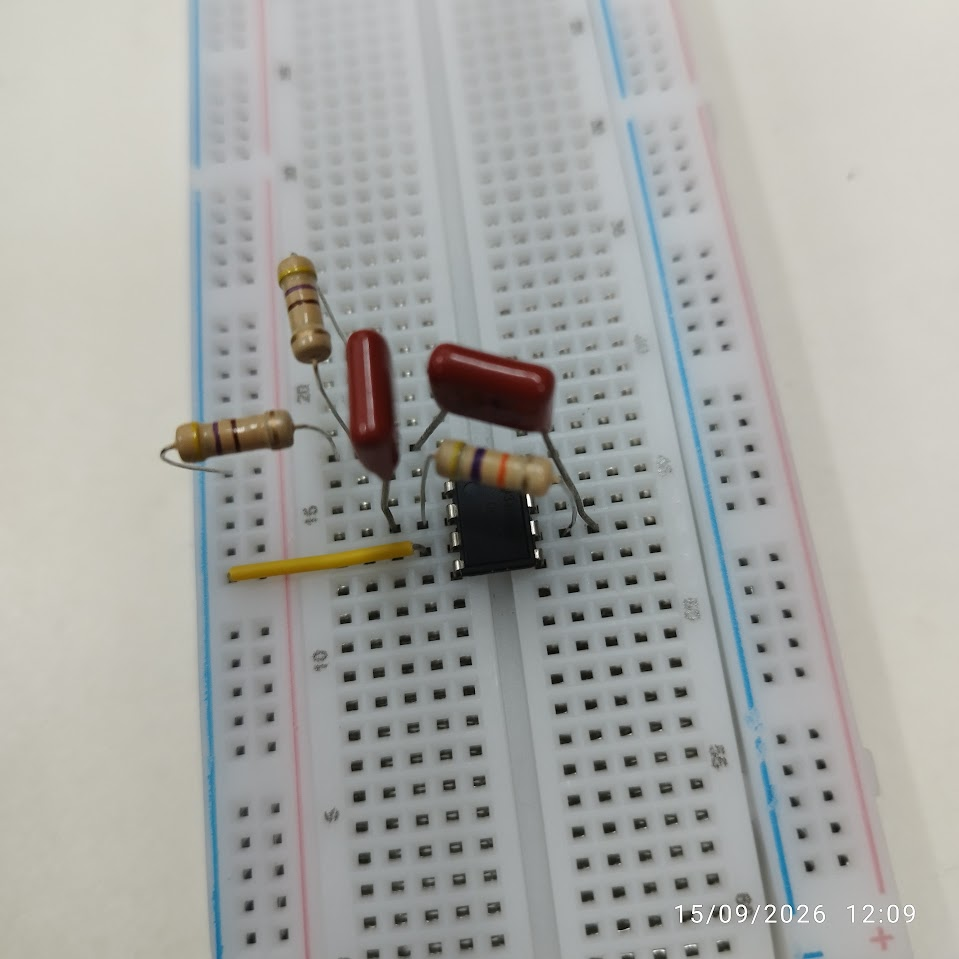
\includegraphics[
        trim=80bp 65bp 65bp 105bp,
        clip,
        width=\linewidth,
        height=0.43\textheight,
        keepaspectratio
      ]{prism-uploads/IMG_20260915_120903.jpg}

      \scriptsize Filtro MFB implementado em protoboard.
    \end{column}
    \hfill
    \begin{column}{0.31\textwidth}
      \centering
      \textbf{Baixa frequência: $40\,\mathrm{Hz}$}

      \vspace{0.08cm}
      \includegraphics[
        page=10,
        trim=150bp 503bp 126bp 145bp,
        clip,
        width=\linewidth,
        height=0.43\textheight,
        keepaspectratio
      ]{prism-uploads/cir02_pratica02_felipeppontes.pdf}

      \scriptsize Saída atenuada e defasagem próxima de $-90^\circ$.
    \end{column}
    \hfill
    \begin{column}{0.31\textwidth}
      \centering
      \textbf{Ressonância: $480\,\mathrm{Hz}$}

      \vspace{0.08cm}
      \includegraphics[
        page=10,
        trim=150bp 252bp 126bp 396bp,
        clip,
        width=\linewidth,
        height=0.43\textheight,
        keepaspectratio
      ]{prism-uploads/cir02_pratica02_felipeppontes.pdf}

      \scriptsize Maior ganho observado na vizinhança da frequência central.
    \end{column}
  \end{columns}

  \vspace{0.18cm}
  \centering\scriptsize Foto do circuito: acervo do autor. Osciloscópio: canal amarelo, saída $V_o$;
  canal verde, entrada $V_i$.
\end{frame}